\chapter{Introduction}
\label{chapter:introduction}
\section{Mathematical Finance}
\label{section:mathematical finance}
Mathematical finance, also known as quantitative finance, is a field of applied mathematics focused on the modeling of financial instruments.
It is rather difficult to overestimate its importance since it is heavily used by investors and investment banks in every day transactions.
In recent decades, this field suffered a complete paradigm shift, following developments in computer science and new theoretical results that enabled investors to better understand the mechanics of financial markets~\citep{compfinance}.

With the colossal sums traded daily in financial markets around the world~\citep{WFE}, mathematical finance has become increasingly important and many resources are invested in the research and development of new and better theories and algorithms~\citep{quants}.


\section{Derivatives}
\label{section:derivatives}
Derivatives are currently one of the subjects most studied by financial mathematicians.
In finance, a \emph{derivative} is simply a contract whose value depends on other simpler financial instruments, known as \emph{underlying assets}, such as stock prices or interest rates.
They can virtually take any form desirable, so long as there are two parties interested in signing it and all government regulations are met.


The importance of derivatives has grown greatly in recent years. In fact, as of June 2017, derivatives were responsible for over \textdollar542 trillion worth of trades, in the Over-the-Counter (OTC) market alone~\citep{BIS}, having started at only \textdollar72 trillion in June 1997, as can be seen in \autoref{fig:OTC} (the OTC market refers to all deals signed outside of exchanges).
This growth peaked in 2008 but stalled after the global financial crisis due to new government regulations, implemented because of the role of derivatives in market crashes~\citep{FT}. It is easy to see that mishandling derivatives can have disastrous consequences. However, when handled appropriately, derivatives prove to be very powerful tools to investors, as we will see shortly.


\begin{figure}[!htb]
    \centering
      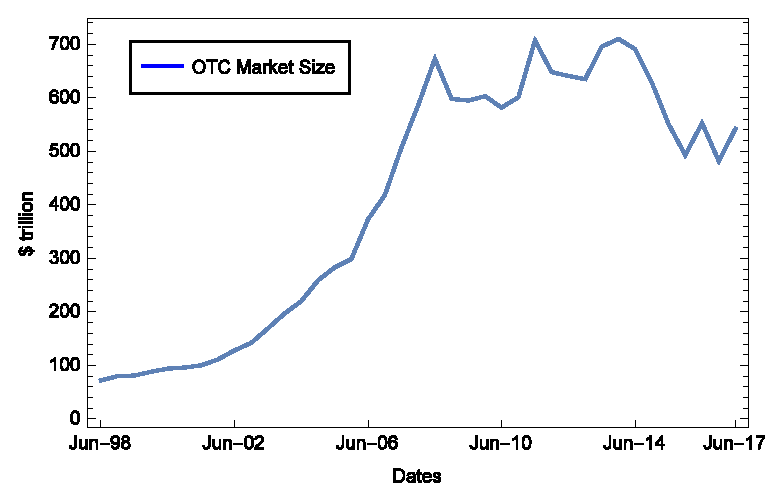
\includegraphics[width=.6\linewidth,trim={2pt 17pt 0 0},clip]{OTC.eps}
      \caption{Size of OTC derivatives market since July 1997.}\label{fig:OTC}
    \end{figure}

\section{Options}
\label{section:options}
Of all classes of derivatives, in this master thesis we will focus particularly on the most traded type~\citep{Hull}: \emph{options}.

As the name implies, an \emph{option} contract grants its buyer the \emph{option} to buy (in the case of a \emph{call} type option) or sell (for \emph{put} options) its underlying asset at a future date, known as the \emph{maturity}, for a fixed price, known as the \emph{strike price}.
In other words, when signing an option, buyers choose a price at which they want to buy/sell (call/put) some asset and a future date to do this transaction. When this date arrives, if the transaction is favorable to the buyers, they exercise their right to execute it.

The description above pertains only to \emph{European} options. In this thesis, this type of contracts will be used for model calibration and validation. Other option types will also be considered, however. We shall approach \emph{American} options, contracts that enable their buyers to exercise their right to buy/sell the underlying asset at any point in time \emph{until} the maturity date. Other less common types, commonly known as \emph{Exotic} options, will also be studied in the following sections, with focus on one of the most common types, known as \emph{Barrier} options.



It's important to emphasize the fact that an option grants its buyer the \emph{right} to do something. If \emph{exercising} the option would lead to losses, the buyer can simply decide to let the maturity date pass, allowing the option to expire without further costs. This is indeed the most attractive characteristic of options.



\subsection{Why Options are Important}
\label{subsection:why options are important}
Options are very useful tools to all types of investors. In simple terms, there exist two types of investors in the market: hedgers and speculators.

To hedgers (i.e. investors that want to limit their exposure to risk), options provide safety by fixing a minimum future price on their underlying assets - e.g. if hedgers want to protect themselves against a potential future price crash affecting one of their assets, they can buy put type options on that asset. With these, even if the asset's value does crash, their losses will always be contained because they can exercise the options and sell the asset at the option's higher strike price.

Options are also very useful to speculators (i.e. investors that try to predict future market movements). The lower price of options when compared to their underlying assets grants this type of investors great leveraging capabilities and, with them, access to much higher profits if their predictions prove right. The opposite is also true, and a wrong prediction can equally lead to much greater losses.

Due to all their advantages, and unlike some other types of derivatives, \emph{options have a price}. Finding the ideal price for an option is a fundamental concern to investors, because knowing their appropriate value can give them a chance to take advantage of under or overpriced options.
Finding this price can be very difficult for some option types, however, and though a lot of research has been done towards this goal, a great deal more is still required.


\section{Volatility}
Volatility is a quantity that greatly affects option prices and is used as a parameter in all pricing models. It's very difficult to define it without the necessary financial background, so we will postpone this description to \autoref{chapter:volatility}, where we will study it in great detail.
For now, we can say that despite its importance, and despite our great efforts to study it, this parameter remains as one of the most elusive phenomena in all of quantitative finance. This elusiveness is mainly caused by our inability not only to predict its future behavior but even actually to accurately measuring it, which clearly gives rise to all sorts of problems when using it in any option pricing model.

Due to its importance, many models have been developed throughout the years in an attempt to model this parameter, with varying degrees of success. We will analyze in detail some of the most famous ones in the following chapters, comparing them with one another.

\section{Repository}
In the development of this thesis we used many original code files, written in MATLAB language, from which we obtained the results shown later. They are available in an online repository, which can be accessed freely at \url{https://github.com/Miguel-Ribeiro-IST/Thesis}.
The code is commented to some degree, to ease the interpretation of all the steps taken.

\vfill
\newpage

\section{Objectives}
The goal of this thesis is to study some of the most commonly used models to forecast volatility. We will approach Dupire's local volatility model and Heston, Static/Dynamic SABR stochastic volatility models. We will begin by clearly defining each model and give some insight regarding their advantages and disadvantages.

We will then train all models in a data set of real European option prices, so that they can best replicate real market behavior.

Afterwards, we will implement each trained model on a Monte Carlo numerical pricer, to obtain some simulated option prices. The models will also be compared with one another, to find which is the most suitable in our case.

Finally, the Monte Carlo pricers will be modified to price Barrier options, as an application example of the models.

\section{Thesis Outline}
In \autoref{chapter:background} we begin by giving some financial background required to understand the posterior sections. We will approach the options' payoff and value functions as well as the Black-Scholes formula and related results.

In \autoref{chapter:volatility} we introduce the concept of volatility, implied volatility, and the Greek Vega. We then describe the models to be used, namely Dupire's local volatility model and Heston, Static/Dynamic SABR stochastic volatility models.

Then, in \autoref{chapter:implementation} we focus on how each model will be implemented, calibrated and validated. We introduce the CMA-ES optimization algorithm, which we will use to calibrate the models, as well as the Monte Carlo numerical pricer, used to estimate option prices with each calibrated model.

Afterwards, in \autoref{chapter:results} we comment the results obtained with each of the models and compare them to one another. We also apply these models to price Barrier options. At the end of this chapter we also present some of the pitfalls found during implementation and how we solved them.

Finally, in \autoref{chapter:conclusions} we give a general overview of the work done and present some of the main conclusions made and possible future work.